%!TEX program = xelatex
%%%%%%%%%%%%%%%%%%%%%%%这是导言部分的开始%%%%%%%%

%========= 导言部分声明文档的类型=================
\documentclass{article}

%=========导言部分可可以加载宏包=================
\usepackage{amsmath}                % 数学公式排版宏包
\usepackage{amssymb}                % 数学符号命令宏包
\usepackage{amsthm}                 % 数学定理宏包
\usepackage[UTF8]{ctex}             % 中文输入宏包
\usepackage[a4paper]{geometry}      % 页面设置宏包
\usepackage{setspace}               % 行间距宏包
\usepackage{graphicx}               % 图片宏包
\usepackage{listings}               % 代码宏包
\usepackage{color}					% 颜色宏包
\usepackage{xcolor}                 % 颜色处理宏包
\usepackage{float}                  % 浮动对象式样宏包
\usepackage{fontspec}
\usepackage{enumerate}				% 列举编号包

%=========页面设置==============================
\geometry{left=1cm,right=1cm,top=1cm,bottom=2cm}
\onehalfspacing
\setlength\parindent{0em}

%=========代码格式设置============================
\definecolor{dkgreen}{rgb}{0,0.6,0}
\definecolor{gray}{rgb}{0.5,0.5,0.5}
\definecolor{mauve}{rgb}{0.58,0,0.82}
% \setmonofont{Consolas}
\lstset{
	numbers = left, 	
	numberstyle = \color{gray}, 
	keywordstyle = \color{blue},
	commentstyle = \color{dkgreen}, 
	stringstyle = \color{mauve},
	basicstyle = \ttfamily,
	breaklines = true,
	frame = shadowbox, % 阴影效果
	rulesepcolor = \color{ red!20!green!20!blue!20} ,
	escapeinside = ``, % 英文分号中可写入中文
	xleftmargin = 2em,xrightmargin=2em, aboveskip=1em,
	framexleftmargin = 2em
} 

%=========导言部分可以定义标题信息===============
\title{组会报告}
\author{徐益}
\date{\today}
%%%%%%%%%%%%%%%%%%%%%%%这是导言部分的结束%%%%%%%%%

%%%%%%%%%%%%%%%%%%%%%%%这是正文部分的开始%%%%%%%%%
\begin{document}

%=========生成标题================================
\maketitle

%=========开始正文的输入==========================

%===========第一节=================
\section{工作内容}
1. 实现多线程系统;

2. 处理部分问题。

%===========第二节=================
\section{多线程系统}
\subsection{系统结构}
\begin{figure}[H]
	\centering
	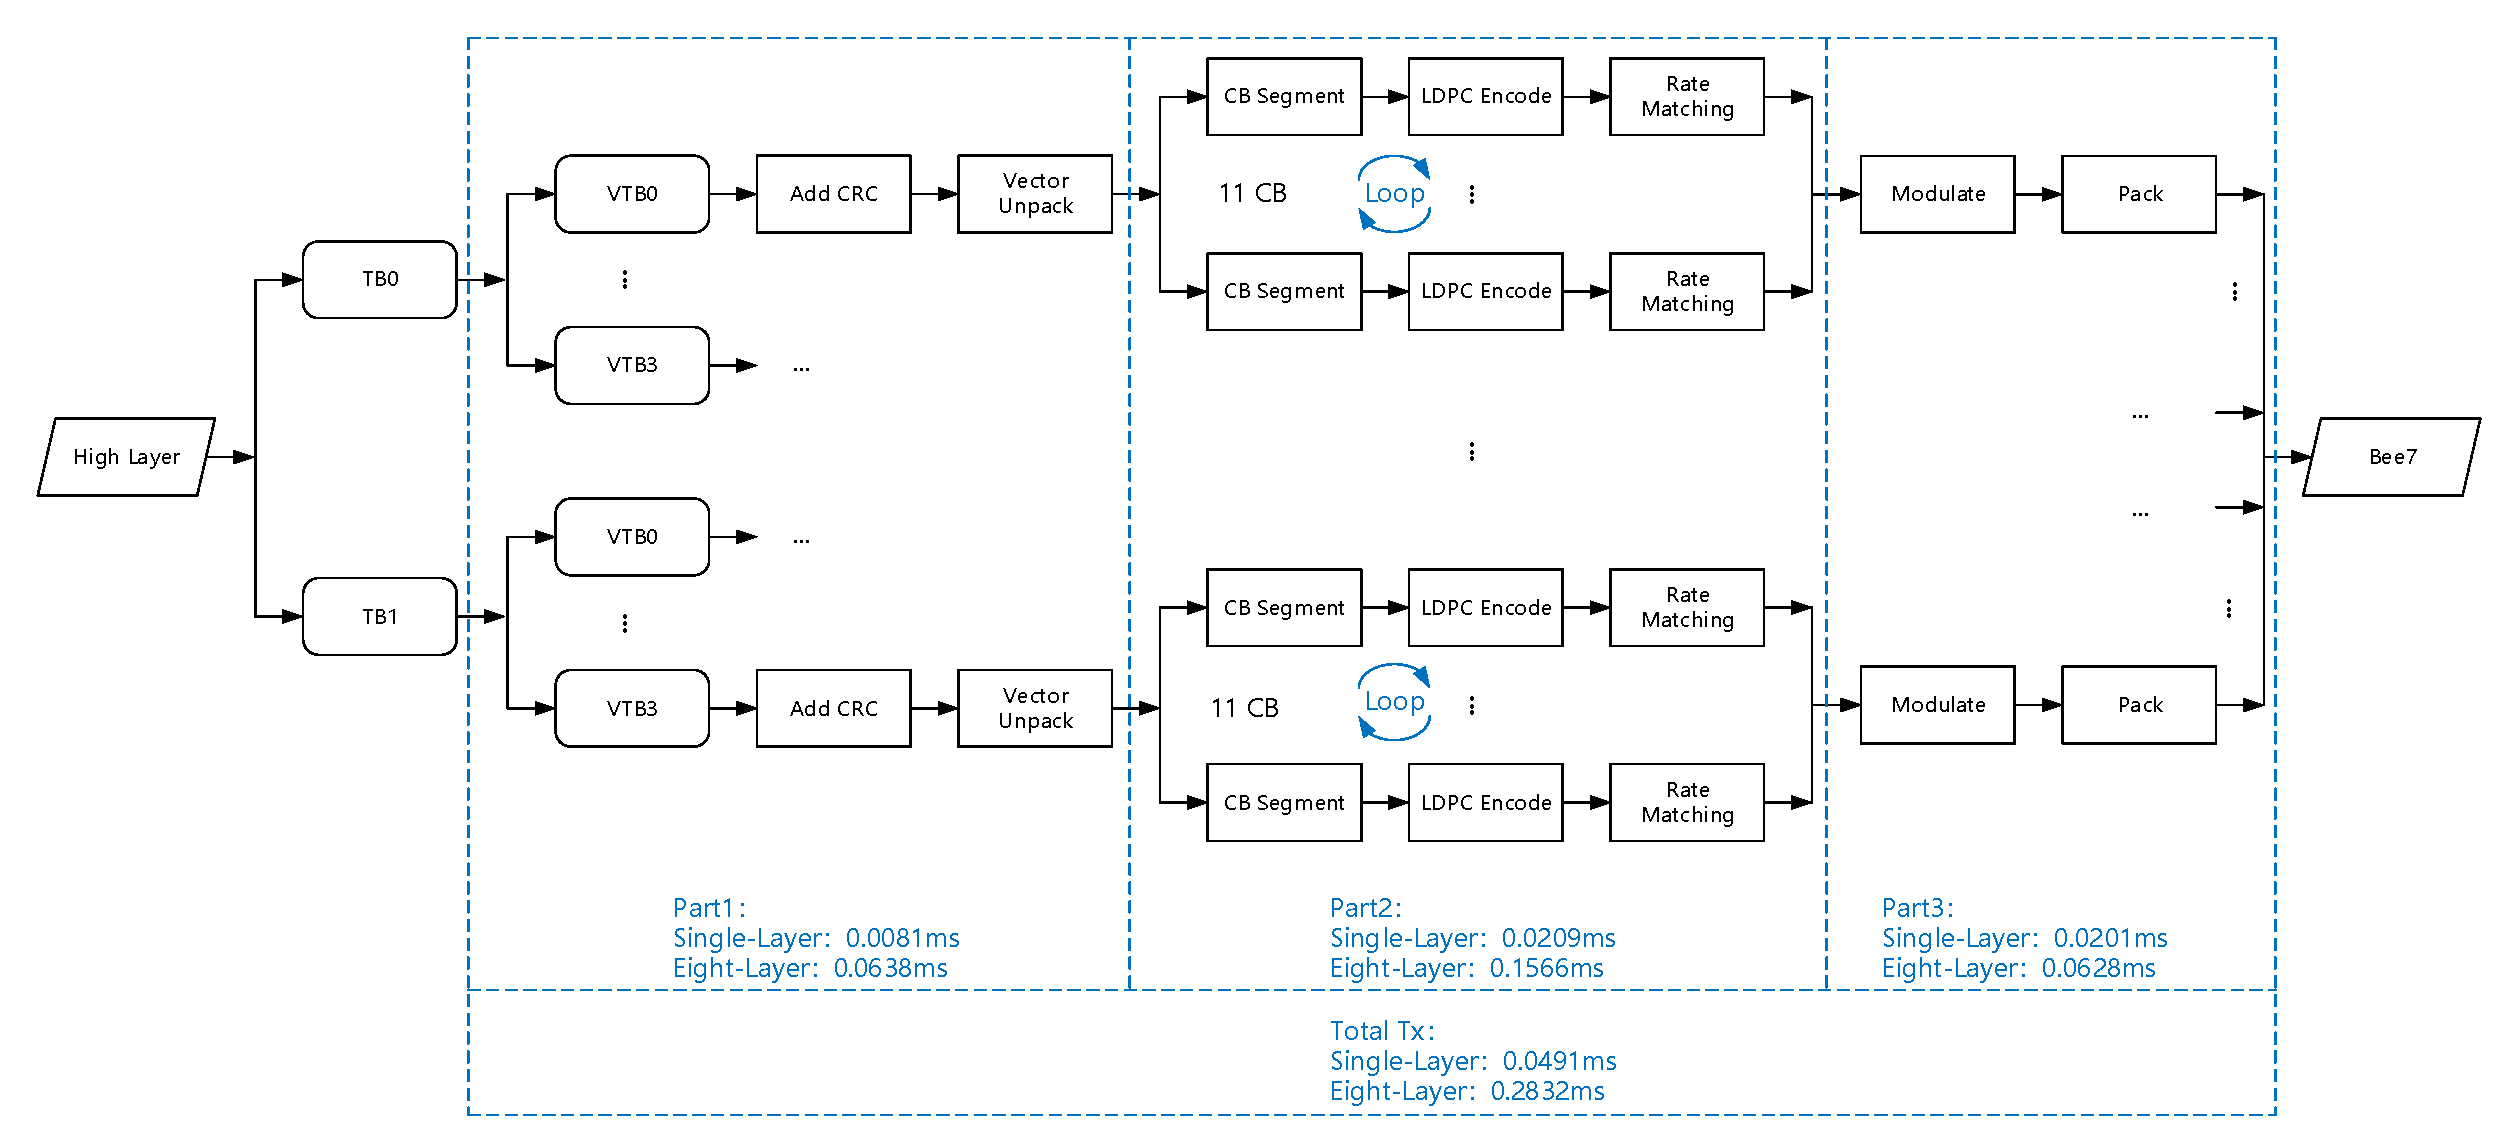
\includegraphics[width = .8\textwidth]{txstr.pdf}
	\caption{发送端}
\end{figure}
\begin{figure}[H]
	\centering
	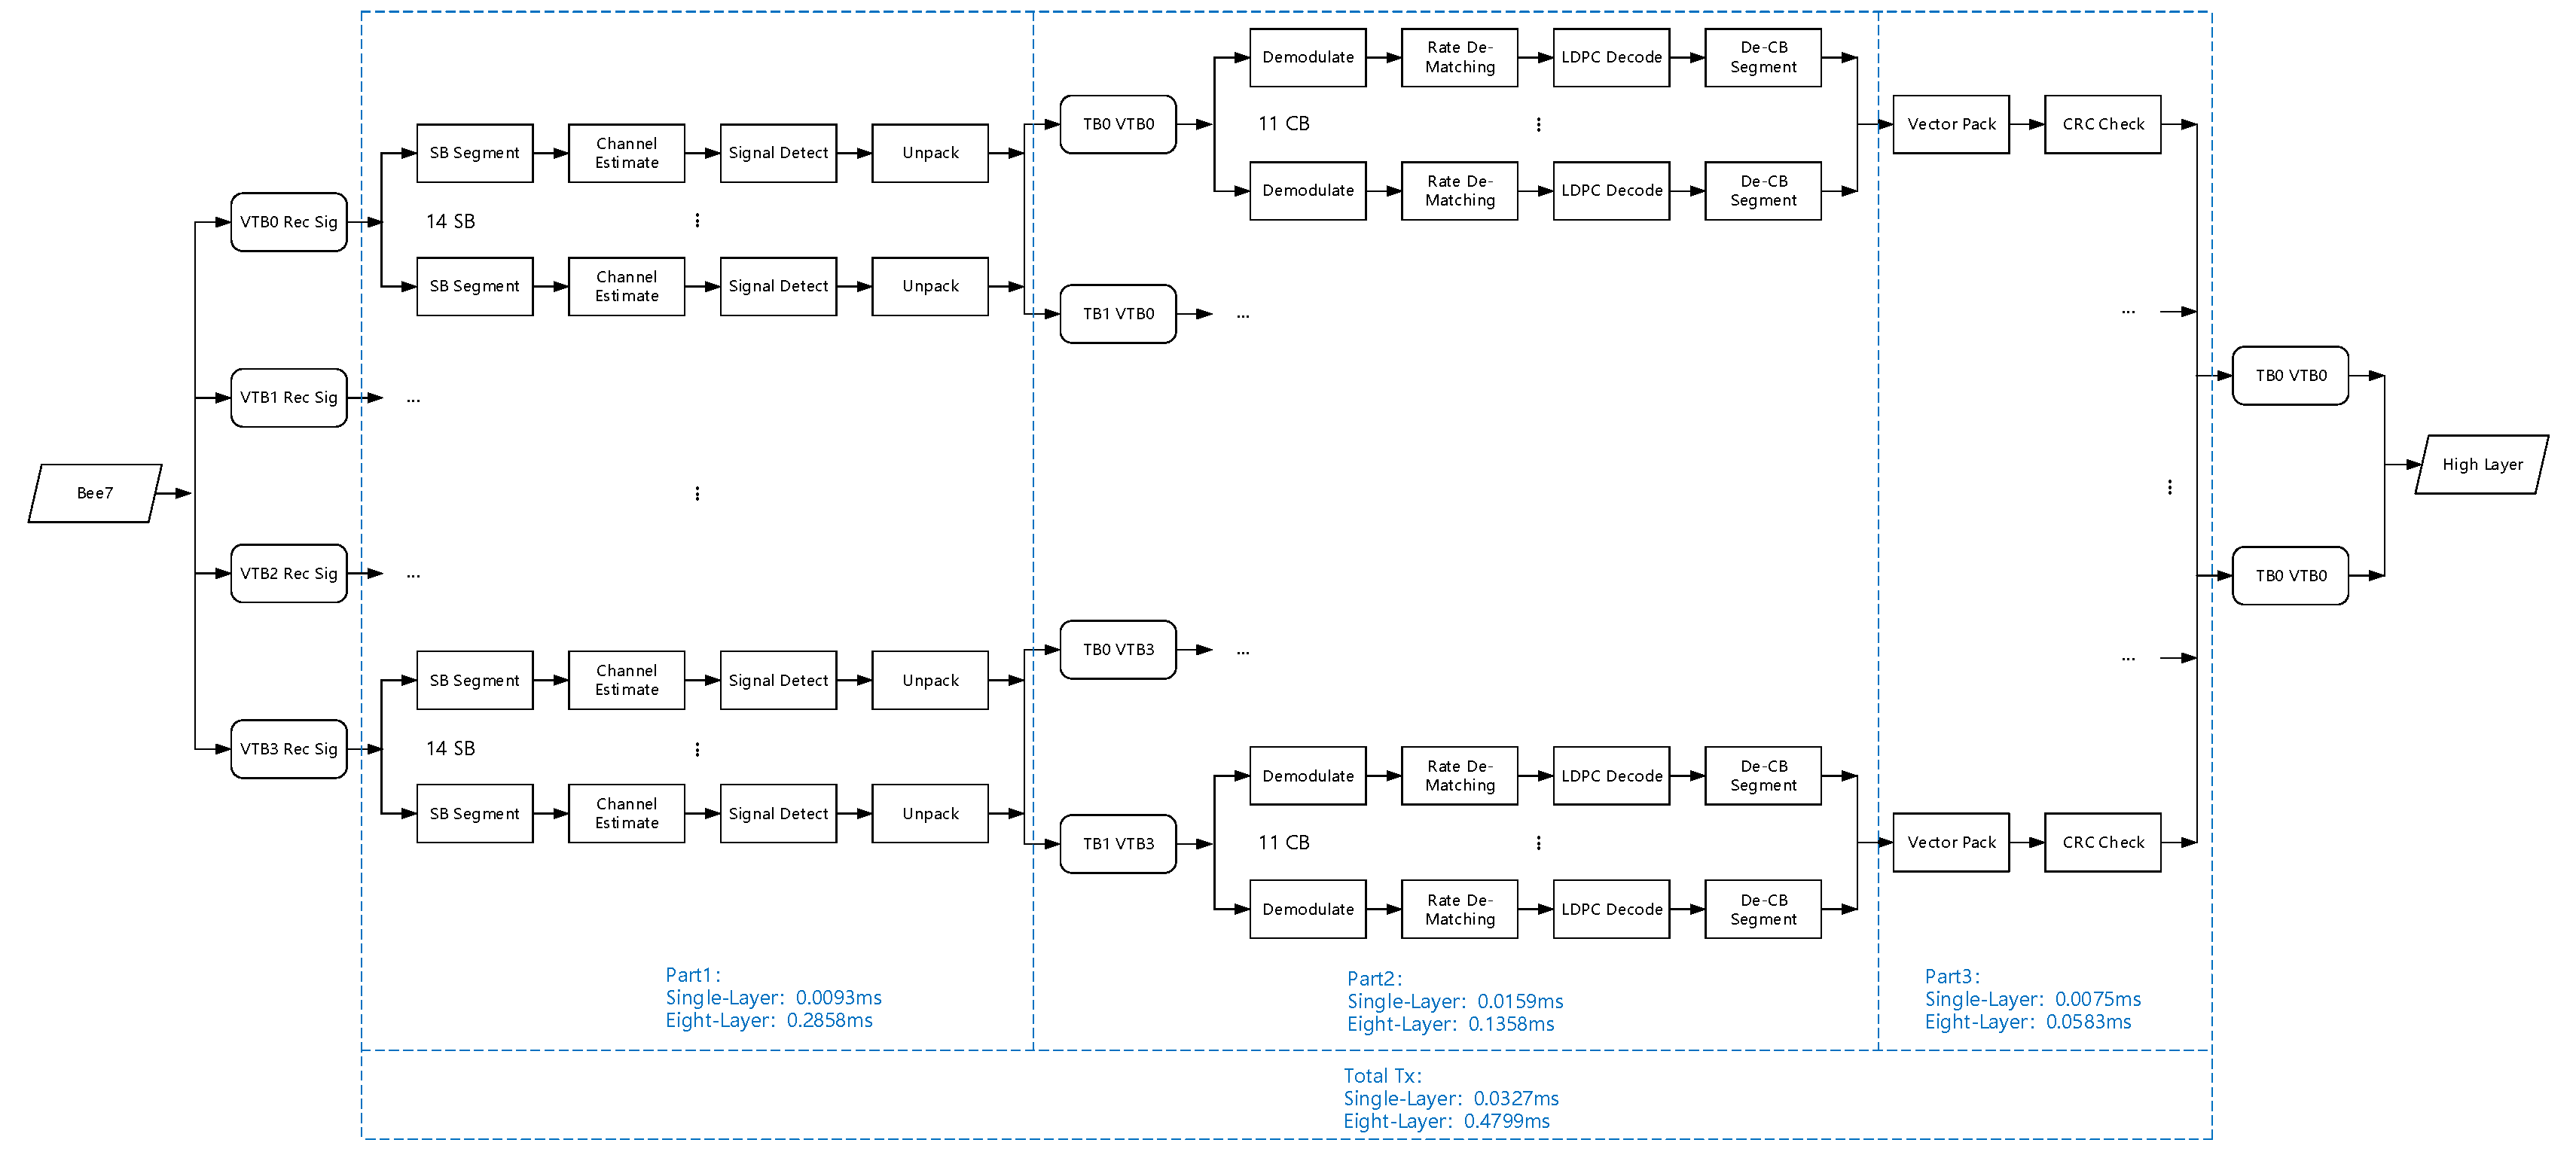
\includegraphics[width = .8\textwidth]{rxstr.pdf}
	\caption{接收端}
\end{figure}
\subsection{测试结果}
\begin{figure}[H]
	\centering
	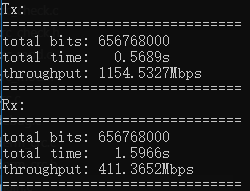
\includegraphics[width = .4\textwidth]{res.png}
	\caption{吞吐量结果}
\end{figure}
\begin{figure}[H]
	\centering
	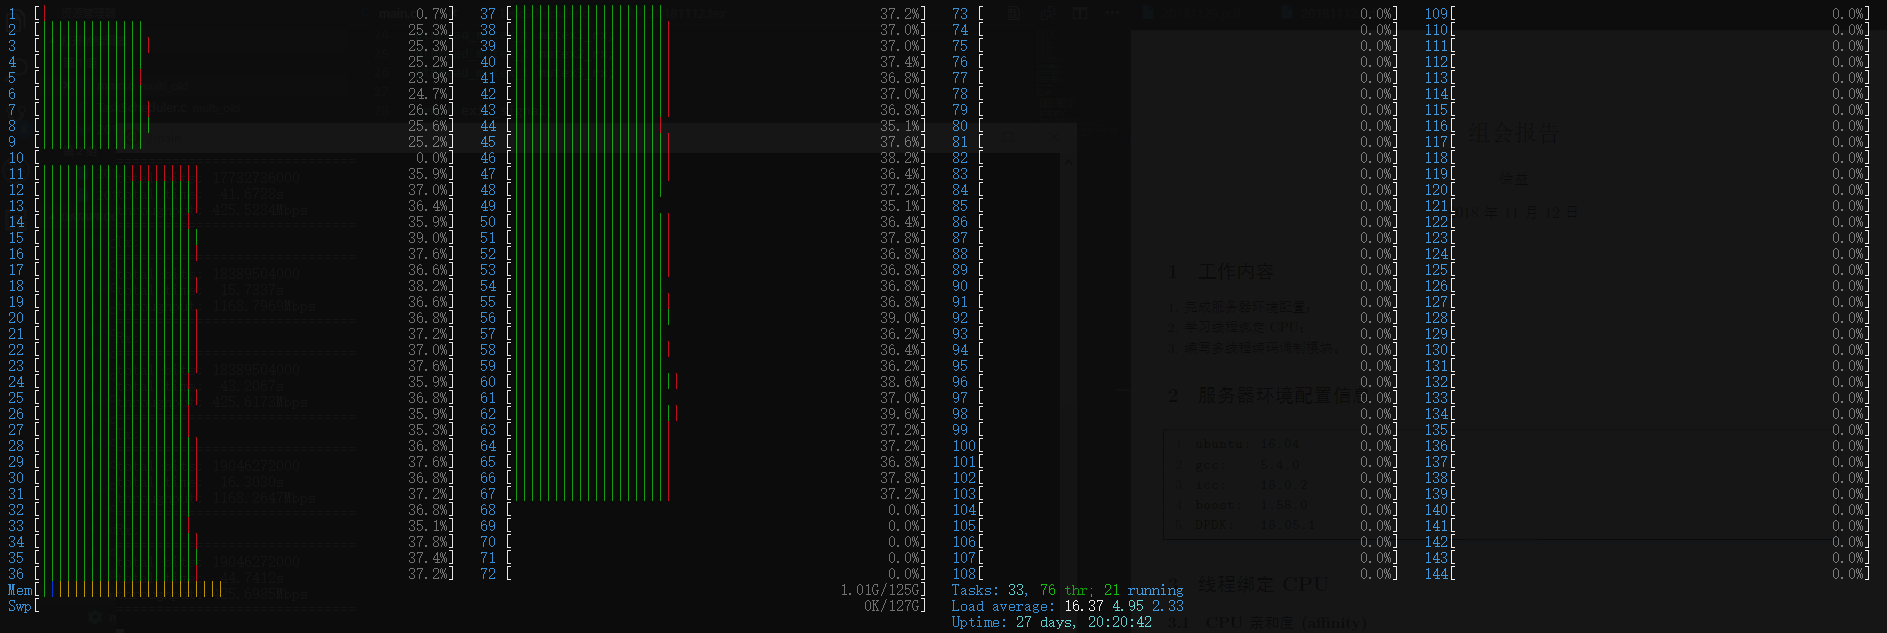
\includegraphics[width = \textwidth]{cpures.png}
	\caption{CPU占用情况}
\end{figure}

%===========第三节=================
\section{已处理的问题}
1. 基于SIMD的LDPC原算法需要重复利用一些内存空间;\\
解决:改写译码器空间结构。

2. 子线程完成时的信号量出现冲突;\\
解决:每个子线程使用不同的信号量。

%===========第四节=================
\section{待解决的问题}
\subsection{模拟信道对收发性能有影响}
\subsubsection{解绑前}
\begin{figure}[H]
	\centering
	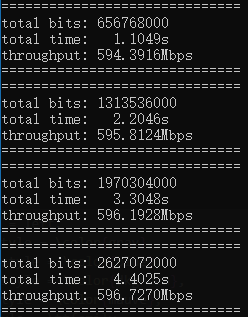
\includegraphics[width = .4\textwidth]{txslow.png}
	\caption{有模拟信道时的发送端性能}
\end{figure}
\begin{figure}[H]
	\centering
	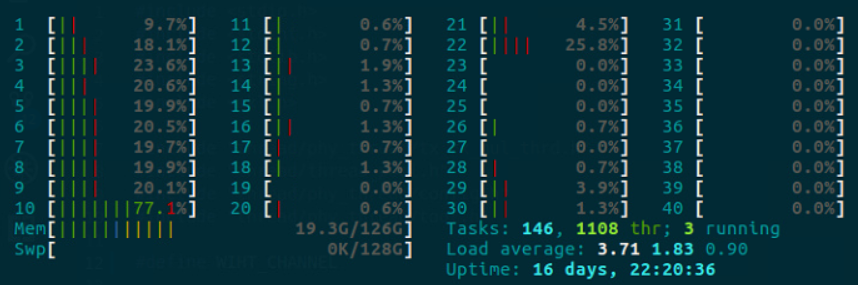
\includegraphics[width = .8\textwidth]{cpuslow.png}
	\caption{有模拟信道时的CPU占用情况}
\end{figure}
\subsubsection{解绑后}
\begin{figure}[H]
	\centering
	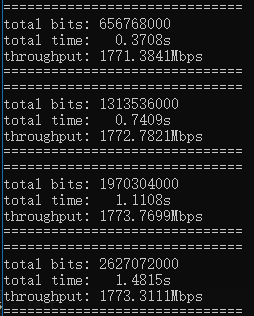
\includegraphics[width = .4\textwidth]{txfast.png}
	\caption{与模拟信道解绑后的发送端性能}
\end{figure}
\begin{figure}[H]
	\centering
	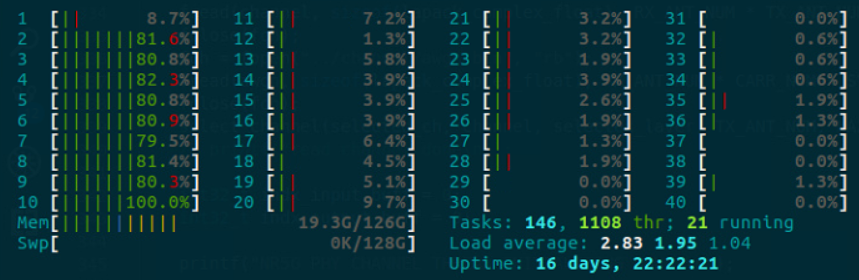
\includegraphics[width = .8\textwidth]{cpufast2.png}
	\caption{与模拟信道解绑后的CPU占用情况}
\end{figure}
\subsubsection{可能的原因和解决方法}
可能的原因:线程的睡眠和再唤醒会对吞吐量造成影响。\\
可能的解决方法:在等待期间用轮询代替睡眠。

\subsection{线程池开得过大对性能有影响}
\subsubsection{TX使用9线程线程池}
\begin{figure}[H]
	\centering
	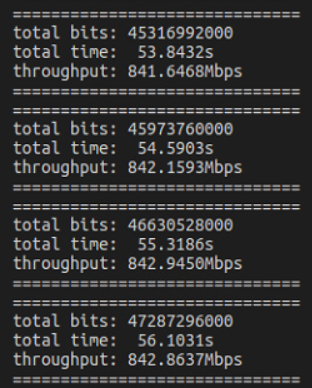
\includegraphics[width = .4\textwidth]{tx9.png}
	\caption{开9线程线程池时的性能}
\end{figure}
\begin{figure}[H]
	\centering
	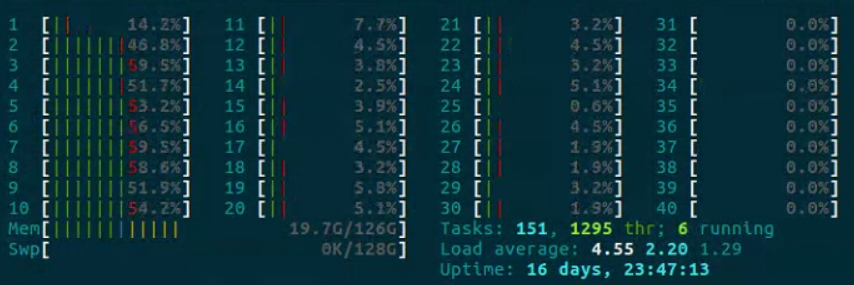
\includegraphics[width = .8\textwidth]{cpu9.png}
	\caption{开9线程线程池时的CPU占用情况}
\end{figure}
\subsubsection{可能的原因和解决方法}
可能的原因:线程池调度对性能有影响。\\
可能的解决方法:查看线程池代码;尝试线程绑定CPU。

\subsection{有一定几率出现线程死锁}
\begin{figure}[H]
	\centering
	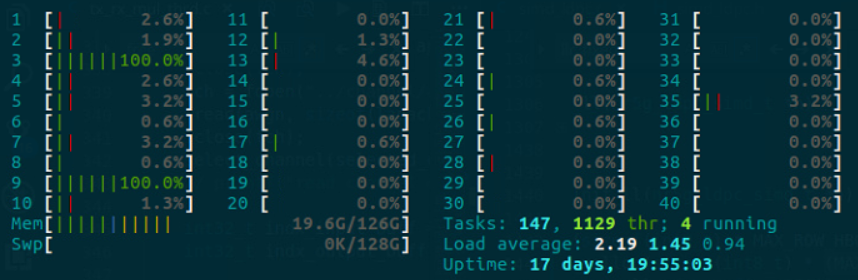
\includegraphics[width = .8\textwidth]{dead.png}
	\caption{死锁的CPU占用情况}
\end{figure}

%===========第五节=================
% \section{5GNR-LDPC报告}


%===========下周计划=================
\section{下阶段计划}
1. 尝试解决上述问题;

2. 准备开题。

\end{document}
%%%%%%%%%%%%%%%%%%%%%%%这是正文部分的结束%%%%%%%%%%%%